

\documentclass[a4paper,11pt]{article} 
\usepackage[spanish]{babel}           
\usepackage[utf8]{inputenc}           

\usepackage[T1]{fontenc}   		   % Fonte por defecto.
\usepackage{graphicx, subfigure}    		   % Engadir imaxes.
\usepackage{color}      		   % Uso de cores.
\usepackage{anysize}     		   % Modificar o tamaño dos marxes.
\usepackage{multicol, multirow}    % Escribir a doble, triple...columna.
\usepackage{bm}          		   % Letras gregas en negriña.
\usepackage{textcomp}    		   % Símbolos, poden consultarse na rede.
\usepackage{eurosym}     		   % Símbolo € (\euro).
\usepackage{amsthm}                % Paquete da AMS para escribir teoremas.
\usepackage{amsmath,amsfonts}      %Paquetes específicos de símbolos.
\usepackage{lineno}                % Numerar as liñas. 

\marginsize{1.5cm}{1.5cm}{1.5cm}{1.5cm} % MARXES: Esq, der, sup, inf.
\parindent=0mm                        % Sangría. 
\parskip=2mm                          % Espazo entre párrafos.
\renewcommand{\baselinestretch}{1}    % Interliñado.
\renewcommand{\spanishtablename}{Táboa} 


\title{Tema 3: Memoria a longo prazo I. Procesos de codificación e consolidación}
\date{}


\begin{document}  

\maketitle 

\section{Introdución ós procesos na MLP}
\begin{itemize}
	\item \textbf{Enfoque procesual:} A memoria é a capacidade dun individuo para adquirir e 				almacenar información, e para recuperar información xa almacenada. 
	\item \textbf{Codificación:} A información presentada a un individuo transfórmase dunha forma
	física (ondas de luz ou son que afectan ós receptores) nunha representación de memoria (trazo de
	memoria ou pegada mnémica). 
	\item \textbf{Almacenamento:} Consiste nos procesos que fan referencia ó conxunto de factores
	que afectan á persistencia temporal da información codificada. Estes procesos poden ser
	construtivos (\textit{exemplo:} repaso) ou destrutivos (\textit{exemplo:} decaemento ou
	interferencia).
	\item \textbf{Recuperación:} A información almacenada pode recuperarse con diferentes obxectivos.
\end{itemize}

\section{A hipótese dos niveis de procesamento: incorporación de novos parámetros e avaliación crítica}
\subsection{O trazo de memoria como resultado dunha codificación múltiple. Estudos pioneiros de Underwood}
Benton Underwood é o primeiro en establecer unha hipótese sobre a multiplicidade de códigos. Suxire que o trazo resultante da codificación dun ítem inclúe atributos de diferentes tipos:
\begin{itemize}
	\item \underline{Temporal}: Permite datar o suceso.
	\item \underline{Espacial}: Sobre todo con información visual.
	\item \underline{De frecuencia}: A modo de ``contador''.
	\item \underline{De modalidade}: Permite discriminar a orixe dos recordos.
	\item \underline{De tipo ortográfico}: Explica as palabras substitutivas no fenómeno da punta da
	lingua.
\end{itemize}

A composición de atributos do trazo de memoria permite discriminar a orixe interna ou externa dos nosos recordos. Os recordos externos adoitan ser máis vívidos, porque conteñen máis atributos contextuais e sensoriais e máis detalles semánticos que os internos. Os internos conteñen máis información sobre operacións cognitivas, como o razoamento, o repaso ou a búsqueda.

\subsection{Multiplicidade de códigos e outros supostos}
\begin{itemize}
	\item \textbf{Organización funcional xerárquizada:} Os niveis máis ``superficiais'' corresponden
	ó procesamento de rasgos físicos, e os máis ``profundos'' ó de propiedades semánticas.
	\item \textbf{Posibilidade de elixir o nivel de procesamento segundo as demandas da tarefa:} A
	codificación dunha palabra non é fixa en tódalas ocasións.
	\item \textbf{Relación funcional entre o nivel de procesamento e a persistencia temporal do
	trazo de memoria:} A maior profundidade xera trazos máis duradeiros.
\end{itemize}

\subsection{O traballo pioneiro de Posner (1969-1978)}
Posner realiza a primeira análise cronométrica dos niveis de procesamento. 

A súa tarefa experimental consiste na presentación visual de dúas letras, que o suxeito debe xulgar como iguais ou diferentes, mentres se rexistra o seu tempo de reacción. Os xuizos de semellanza realízanse segundo tres modalidades:
\begin{itemize}
	\item[-] Identidade física (A A).
	\item[-] Identidade nominal (A a).
	\item[-] Igualdade semántica ou xuizo categorial (A e, vogais).
\end{itemize}

Os resultados amosan que o tempo de reacción é menor para a identidade física que para a nominal e a semántica.

\subsection{A formulación orixinal de Craik e Lockhart (1972)}
Critican as teorías multialmacén, alonxándose da idea de almacéns de memoria que posúen códigos específicos e enfatizando que a forma de manipular o material determina a súa durabilidade na MLP.

Así, propoñen a hipótese dos niveis de procesamento: a análise perceptiva dun ítem implica un continuo de niveis de procesamento, que comeza nos máis ``superficiais'' (análise de rasgos físicos ou sensoriais) e acada os máis ``profundos'' (codificación das propiedades semánticas da información). 

O resultado deste proceso e a aparición un trazo de memoria cuxa persistencia depende do nivel de codificación. Surxen así dous tipos de procesamento: o tipo I (repaso de mantemento) e o tipo II (repaso de elaboración). 

Máis tarde, Craik e Tulving (1975) realizan experimentos nos que os participantes deben emitir tres tipos de xuízos sobre algunhas palabras, sendo estes sobre letras, rimas ou de tipo semántico. Despois enfróntanse a unha lista da que deben seleccionar as palabras vistas nas probas anteriores. Os investigadores conclúen que canto máis profundo é o nivel de procesamento, maiores son o tempo de reacción e a probabilidade de recordo posterior. 

\subsection{Modificacións na formulación orixinal. Incorporación de novos parámetros}
\begin{itemize}
	\item \textbf{Elaboración:} Riqueza, extensión ou amplitude da codificación dentro dun
	determinado nivel (compoñente cuantitativo). Para o mesmo nivel de procesamento o recordo depende
	do número de operacións de codificación realizadas.
	\item \textbf{Distintividade:} Grao de discriminabilidade dun trazo de memoria no contexto
	representacional. Recordarase mellor un ítem cando o trazo posúa propiedades únicas respecto ós
	demais ítems a aprender. 
	\item \textbf{Congruencia:} Nas tarefas semánticas, cando os ítems son positivos, frase e
	palabra son semanticamente congruentes e forman unha unidade cognitiva. Cando son negativos
	codifícanse por separado.
	\item \textbf{Destreza:} O recordo da información tamén depende das habilidades cognitivas dos
	individuos. 
\end{itemize}

\subsection{Avaliación crítica da hipótese dos niveis}
\begin{enumerate}
	\item Non existe unha medida da profundidade de procesamento que sexa independente, isto é, non 		pode facerse unha verdadeira medida empírica do constructo. A asociación de profundidade e 				latencia de codificación aporta malos resultados, xa que o tempo de reacción non só está modulado 	pola codificación cuantitativa, senon tamén pola elaboración. Ademais, definir os niveis de 			profundidade en termos de recordo peca de circularidade.
	\item Non se demostrou que a profundidade sexa unha dimensión continua. Só pode dicirse que hai
	unha diferenza estable entre as tarefas de procesamento semántico e as de codificación
	perceptiva.
	\item A  hipótese dos niveis comparte algúns principios coas teorías multialmacén. Así, os niveis 	apóianse nunha concepción lineal do procesamento, polo que se pode cuestionar a súa organización
	xerárquica.
	\item A teoría recalca un sesgo, pouco xustificado, cara os procesos de codificación, e descoida
	os de recuperación. Porén, o recordo depende tanto das condicións de codificación como do
	contexto no que se recorde.
	\item Existen relacións imprecisas entre os niveis e o recordo. Destacamos dúas prediccións que
	non contan co apoio empírico total, porque non sempre ocorren:
	\begin{enumerate}
		\item ``A mera repetición de información procesada no mesmo nivel non incrementa o recordo''.
		A repetición pode mellorar a retención, sobre todo en recoñecemento.
		\item ``Canto máis profunda sexa a codificación, mellor será o recordo''. As características 			da proba de memoria poden afectar á eficacia da codificación, coma no principio de 						procesamento apropiado para a transferencia.
	\end{enumerate}	
	\item O constructo ``niveis de procesamento'' non xera grandes desenvolvementos teóricos. É moi
	descritivo, pero non aporta mecanismos que expliquen a hipótese.
\end{enumerate}

\subsubsection{O principio do <<procesamento apropiado para a transferencia (PAT)>>}
Postula que para que unha proba (test) poida poñer de manifesto o coñecemento previo, os requisitos de procesamento de dita proba deben coincidir coas condicións de procesamento da codificación. Este principio nace para explicar o fenómeno da profundidade do procesamento.

En 1977, Morris, Bransford e Franks poñen a proba o principio, examinando se a retención está determinada polo que os individuos fan durante a codificación ou pola medida en que os requisitos de procesamento durante o test coinciden coa codificación. Deseñan unha tarefa na que os participantes deben facer un xuízo fonolóxico ou semántico sobre cada ítem dunha lista de palabras, pero non os informan de que logo deberán recordar esas palabras. Deste xeito a aprendizaxe ocorre accidentalmente, co que se reduce o uso de estratexias de aprendizaxe.

O recordo ponse a proba mediante un de dous test: unha proba de recoñecemento estándar, na que se inclúen as palabras presentadas e un número idéntico de palabras non presentadas; ou unha proba na que se presenta unha serie de palabras e se pregunta se se presentou algunha que rimara con elas. 

Os resultados da primeira proba amosan que un procesamento máis profundo leva a un maior rendemento, o que secunda os resultados de Craik e Tulving. Porén, a segunda proba demostra o contrario: a tarefa de codificación máis superficial leva a unha mellor execución.

Un estudo posterior de Fisher e Craik (1977) replica estes resultados, pero enfatiza a vantaxe xeral dun procesamento máis profundo. Porén, ambos grupos de autores coinciden en que só ten sentido falar da eficacia dun método de aprendizaxe no contexto do tipo de proba final (aquela que pon a proba o recordo).


\section{Organización e recordo}
%\subsection{Importancia da organización: perspectiva histórica}
\subsection{Evidencia experimental da importancia da organización}
\begin{itemize}
	\item \underline{Organización dentro do material de estímulo}: Os suxeitos son quen de aproveitar
	a organización do material proporcionada polo experimentador, a chamada organización externa
	(porque ven imposta de fóra). Isto refléxase tanto nas puntuacións de recordo coma no agrupamento
	das respostas durante o recordo.
	 
	Dentro desta organización distínguense tres tipos:
	\begin{itemize}
		\item \textbf{Asociativa:} Refléxase na agrupación asociativa no recordo.
		\item \textbf{Categórica:} O suxeito emprega as categorías taxonómicas da selección de
		palabras para agrupar e recordar a lista máis facilmente.
		\item \textbf{Xerárquica:} Recórdase mellor o material organizado xerarquicamente que o que
		se presenta entremezclado.
	\end{itemize}
	\item \underline{Organización subxectiva do material azaroso}: Os suxeitos tentan organizar o
	material aleatorio para recordalo mellor (``esforzo por atopar un sentido'' de Bartlett). Isto
	é demostrado por Tulving, que presenta ós seus suxeitos listas de palabras non relacionadas e
	ordeadas de forma aleatoria, e obtén que a orde coa que os suxeitos as recordan é cada vez máis
	estereotipada, co que aumenta o grao de organización subxectiva. Estes agrupamentos tenden a 			reflexar variables semánticas.
	\item \underline{Instruccións para organizar}: Danse instruccións ós suxeitos para que organicen
	o material de varios xeitos, e logo pídeselles que recorden dito material. De novo, a aprendizaxe
	é accidental.
	
	A organización, neste caso, pode ser de tres tipos:
	\begin{itemize}
		\item \textbf{Categorización semántica:} A organización de palabras en categorías produce
		resultados tan bós como cando se aprenden porque si.
		\item \textbf{Seriación:} Organización secuencial ou serial dos ítems, xa moi valorada na 				época clásica. Adoita empregarse cando se quere aprender un conxunto completo de ítems, e é 			sinxelo utilizala se os ítems se presentan na mesma orde en cada ensaio. Esta estratexia 				asegura o recordo de tódolos ítems, evitando os olvidos que adoitan darse no recordo libre.
		\item \textbf{Formación de imaxes visuais:} Atopamos tres técnicas.
		\begin{itemize}
			\item \underline{Método dos lugares}: É a base de moitas técnicas mnemónicas, e comeza a
			empregarse xa na antigua Grecia. Funciona sobre todo cando os ítems a recordar poden 					transformarse facilmente en imaxes, coma no caso de palabras concretas, aínda que tamén
			favorece o recordo de palabras abstractas. 
			
			Esta estratexia ten limitacións no recordo de listas, porque non é posible lembrarse dun
			ítem ó azar sen analizar as imaxes visuais dos ítems que o preceden. Algúns 							investigadores tamén opinan que non é útil á hora de aprender material no mundo real.
			\item \underline{Técnica das palabras percha}: Permite lembrar en orde secuencias de
			polo menos dez ítems non relacionados (crese que ata o dobre dos que lembraríamos 						normalmente). Faise seleccionando un número de palabras percha, que rimen cos números de 				un a dez, equivalente ó número de palabras a recordar. Logo créanse imaxes visuais de 					cada palabra da lista en interacción coa súa correspondente palabra percha. 
			
			Para que sexa efectiva, esta técnica require de moito adestramento previo. Ademais, é
			moito máis sinxelo usala con palabras concretas que abstractas, e tamén existen dúbidas
			sobre a súa utilidade na vida cotiá.
			\item \underline{Recordo de nomes}: Consiste en tratar de transformar o nome dunha
			persoa nunha imaxe visual coñecida, para tratar de relacionala coas características
			máis destacables do seu rostro. 
			
			Está demostrado que un breve adestramento con esta técnica mellora moito o recordo, case 				nun 80\%. Con todo, non se asegura a súa efectividade fóra do laboratorio. 
		\end{itemize}		 	
	\end{itemize}
\end{itemize}

\subsection{Técnicas mnemónicas (mnemotecnias)}
Consisten na organización significativa e consciente da información, para poder recordala mellor. Poden engadir un código de memoria adicional ó código orixinal, co que permiten dúas posibles vías de recuperación (\textit{exemplo:} a música facilita o recordo de lemas publicitarios). Son útiles sobre todo para memorizar información arbitraria, porque lle aportan un significado. Deste xeito, permiten unha codificación máis eficaz.

Diferenciaremos entre mnemotecnias internas, que son as que empregamos para recordar algo sen axuda, e externas, como son as axendas, ordenadores, móbiles, alarmas, etc.

Dentro destas existen diferentes técnicas:
\begin{itemize}
	\item \textbf{Técnicas de elaboración:} Enriquecen o material a recordar ó vinculalo cos
	coñecementos previos. Poden ser:
	\begin{itemize}
		\item \underline{Mnemotecnias verbais}: Codificación semántica mediante a asociación de 				letras e ítems a recordar, a veces combinada con ritmos e rimas. Tamén se emprega moito o
		método da historieta, no que se conectan as palabras a lembrar creando unha historia con
		elas.
		\item \underline{Mnemotecnias baseadas na formación de imaxes visuais}: Método dos lugares, 			técnica das palabras percha e recordo de nomes.
	\end{itemize}
	\item \textbf{Técnicas de reducción:} Inversas ás de elaboración, reducen a cantidade de
	información almacenada. A vantaxe fronte ás outras é que poden repasarse moi rapidamente e así
	manterse na memoria mentres se executa outra tarefa (\textit{exemplo:} acrónimos).
	\item \textbf{Axudas externas:} Son de uso obrigado para persoas maiores ou pacientes con dano
	cerebral, aínda que o resto da poboación adoita apoiarse moito nelas (\textit{exemplo:} notas,
	listas, axendas...). 
\end{itemize}

As mnemotecnias axudan melloran o recordo porque nos permiten facer uso dos coñecementos previos. Ademais deste motivo, Ericsson (1988) propón outros tres principios:
\begin{enumerate}
	\item \underline{Codificación significativa}: A información procésase de xeito que sexa
	significativa e teña sentido, relacionándoa co coñecemento previo.
	\item \underline{Estrutura da recuperación}: As pistas que axudan no recordo almacéanse xunto coa
	información a recordar.
	\item \underline{Velocidade}: A práctica prolongada fai que os procesos involucrados na
	codificación e na recuperación funcionen cada vez máis rápido. 
\end{enumerate}

\section{Procesos de consolidación}
Relaciónanse coas fases de codificación e almacenamento, e son determinantes para a retención a longo prazo.

A \textbf{consolidación} é o proceso que permite a existencia relativamente estable dunha pegada de memoria, máis alá do momento actual, e que ocorre de forma gradual e máis ben autónoma. Este proceso desenvólvese ó longo do tempo (non instantaneamente), comezando coa codificación da experiencia. Culmina despois dalgún tempo, en períodos que varían desde minutos ata días, meses ou anos.

Existen dous tipos de consolidación:
\begin{itemize}
	\item \underline{Sináptica}: Ocorre cando se producen cambios estruturais nas conexións
	sinápticas entre neuronas. Apóiase en procesos biolóxicos e pode tardar desde horas ata días en
	completarse. Ata que se completan os cambios, os recordos seguen sendo vulnerables. 
	\item \underline{Sistémica}: Ocorre cando a dependencia da memoria se despraza, de forma gradual,
	desde o hipocampo cara a cortiza, o que se logra reactivando recurrentemente as áreas cerebrais
	implicadas na experiencia inicial (é dicir, repetindo os distintos compoñentes dun recordo) ata 
	que se interconectan e crean o recordo orixinal. En humanos, o proceso pode tardar anos en
	completarse, e os recordos son máis vulnerables ata que non se independizan do hipocampo.
\end{itemize}

\begin{figure}[h!]
	\centering
	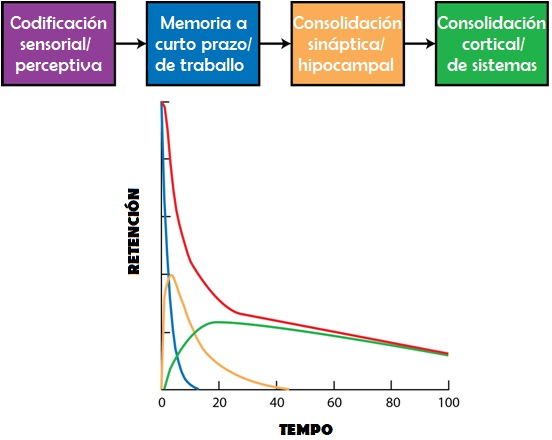
\includegraphics[width=0.45\linewidth]{memoria3_1}
	\caption{Traxectoria da dispoñibilidade dunha pegada de memoria tras varios procesos de 				consolidación}
\end{figure}

Atópanse dous factores moduladores dos procesos de consolidación:
\begin{itemize}
	\item \textbf{O estado emocional do organismo:} Un nivel de activación elevado pode optimizar o
	proceso.
	\item \textbf{O sono:} Existe un momento óptimo para o proceso, que se corresponde cos períodos
	de sono. Aínda que hai poucas evidencias de que se poida aprender mentres se durme, si se valora
	a importancia do sono na consolidación da memoria do que se aprendeu.
\end{itemize}

A reconsolidación demostra que as pegadas de memoria estables e consolidadas son susceptibles de sufrir modificacións cada vez que se lembran (reactivación). Unha vez modificadas, estas pegadas reactivadas volven ser fixas e estables. 

Este proceso podería empregarse de forma práctica en persoas que teñen recordos perturbadores do seu pasado (\textit{exemplo:} desorde de estrés postraumático). Así podería eliminarse o compoñente emocional dun recordo sen alterar o cognitivo.


\end{document} %Non pode haber nada escrito despois desta instrución.
